\section{Identification of the most important variables}

To determine the most significant features, we employed the 
\emph{Feature Importance Widget} from Orange Data 
Mining~\parencite[]{2015:odm}. This tool analyzes the provided data
to calculate the contribution of each feature towards the 
prediction, thereby assessing its impact on the target variable.

\begin{figure}[H]%
    \caption{Feature Importance per Model}%
    \label{fig:fi_importance_per_label}%
    \centering
    \subfloat[\centering Catboost]{{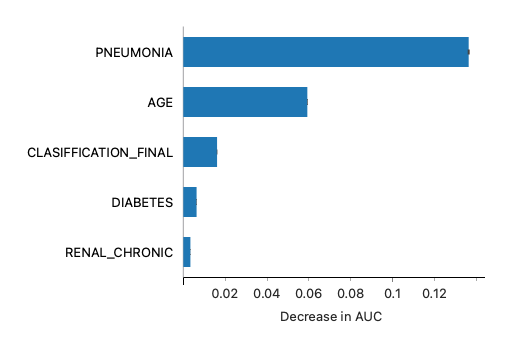
\includegraphics[width=0.45\textwidth]{img/importantvariables/FI_GB_AUC_5.png} }}%
    \qquad
    \subfloat[\centering Neural Network]{{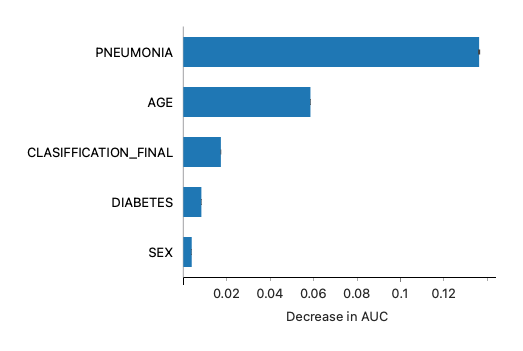
\includegraphics[width=0.45\textwidth]{img/importantvariables/FI_NN_AUC_5.png} }}%
    \qquad
    \subfloat[\centering Random Forest]{{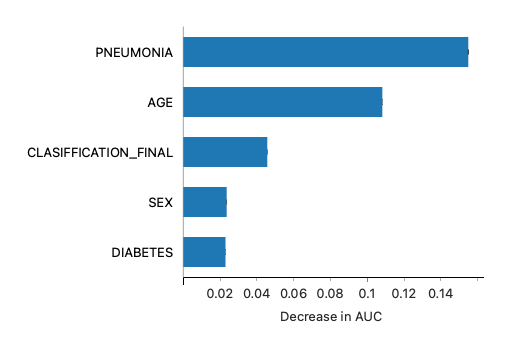
\includegraphics[width=0.45\textwidth]{img/importantvariables/FI_RF_AUC_5.png} }}% 
\end{figure}

Based on the variable rankings presented in Figure~\ref{fig:feat_rank_5}, we 
can observe that the models have identified the variables in alignment with 
our expectations. This comparison confirms that the models are accurately 
prioritizing the variables as anticipated. We identified 4 main variables 
that could affect if a patient with COVID-19 needs to be hospitalized or not:
\begin{itemize}
    \item Pneumonia;
    \item Age;
    \item Classification Final;
    \item Diabetes.
\end{itemize}

\subsection{Pneumonia}

Pneumonia is a serious and common complication of COVID-19, especially in 
severe cases. When someone is infected with the virus that causes COVID-19,
 the infection can spread to the lungs, leading to 
pneumonia. This is the main indicator the a Patient needs to be hospitalized 
urgently. 

\subsection{Age}
Age is a significant factor in the impact and outcomes of COVID-19 infection.
The risk of severe illness from COVID-19 increases with age, with older adults
being at the highest risk for severe illness, complications, and mortality.

\subsection{Classification Final}
The term `Classification Final' pertains to the COVID testing result of a 
patient. As expected, this is a crucial factor because a positive test result
is necessary for a patient to be treated for COVID-19.

\subsection{Diabetes}

People with both type 1 and type 2 diabetes are more likely to have severe 
illness and complications from COVID-19 compared to people without diabetes. 
his increased risk can be attributed to several factors, such as:
\begin{description}
\item[Immune System Impairment] Diabetes can weaken the immune system, 
making it less able to fight off infections;
\item[Coexisting Conditions] people with diabetes often have other 
conditions such as hypertension, cardiovascular disease, or obesity, 
which are themselves risk factors for severe COVID-19
\end{description}
